%%%%%%%%%%%%%%%%%%%%%%%%%%%%%%%%%%%%%%%%%%%%%%%
%%%This is a science homework template. Modify the preamble to suit your needs. 
%The junk text is   there for you to immediately see how the headers/footers look at first 
%typesetting.

\documentclass[12pt]{article}

%AMS-TeX packages
\usepackage{amssymb,amsmath,amsthm} 
\usepackage{commath}
\usepackage[margin=1in]{geometry}
\usepackage{graphicx,ctable,booktabs}
\usepackage[retainorgcmds]{IEEEtrantools}
\usepackage{cancel}
\usepackage{wrapfig}
\usepackage{braket}
\usepackage{enumitem}
\usepackage{pdfpages}
\usepackage{subcaption}
\usepackage{xurl}

\usepackage{graphicx}
\usepackage{subfig}

%Redefining sections as problems

\makeatletter
\newenvironment{problem}{\@startsection
	{section}
	{1}
	{-.2em}
	{-3.5ex plus -1ex minus -.2ex}
	{2.3ex plus .2ex}
	{\pagebreak[3]%forces pagebreak when space is small; use \eject for better results
		\large\bf\noindent{Problem }
	}
}
{%\vspace{1ex}\begin{center} \rule{0.3\linewidth}{.3pt}\end{center}}
	\begin{center}\large\bf \ldots\ldots\ldots\end{center}}
\makeatother

%Fancy-header package to modify header/page numbering 

\usepackage{fancyhdr}
\pagestyle{fancy}
\lhead{Problem \thesection}
\chead{} 
\rhead{\thepage} 
\lfoot{\small\scshape PHYS 600} 
\cfoot{} 
\rfoot{\footnotesize HW 3} 
\renewcommand{\headrulewidth}{.3pt} 
\renewcommand{\footrulewidth}{.3pt}
\setlength\voffset{-0.25in}
\setlength\textheight{648pt}
\allowdisplaybreaks

\newcommand{\partder}[3]{\ensuremath{\left(\frac{\partial {#1}}{\partial {#2}}\right)_{#3}}}

\newcommand{\braks}[1]{\ensuremath{\left\langle{#1} \right\rangle} }

\newcommand{\Omx}[1]{\ensuremath{\Omega_\mathrm{#1} } }
\newcommand{\rhox}[1]{\ensuremath{\rho_\mathrm{#1} } }

\setlength{\parindent}{0pt} % No indent by default

%%%%%%%%%%%%%%%%%%%%%%%%%%%%%%%%%%%%%%%%%%%%%%%

%
%Contents of problem set
%    

\begin{document}
	
	\title{PHYS 600: Homework 3}
	\author{Yarone Tokayer}
	\date{October 8, 2023}
	
	\maketitle
	
	\thispagestyle{empty}

	\begin{problem}{Reviewing the Background}
		\begin{description}
			\item[Density Parameters] In general, $\rhox{m}$ scales as $(1+z)^3$ and $\rhox{\Lambda}$ is constant.  We can now evaluate the desired quantities: \begin{align*}
				\Omx{m}(z=0.5) &= \frac{\rhox{m}(z)}{\rhox{c}(z)}
				\\
				&= \Omx{m,0} (1+z)^3 \frac{ H_0^2 }{H^2(z)}
				\\
				&= \frac{ \Omx{m,0} (1+z)^3 }{ \Omx{m,0}(1+z)^3 + \Omx{r,0}(1+z)^4 + \Omx{k,0}(1+z)^2 + \Omx{\Lambda} }
				\\
				&= \frac{ 0.3 \cdot (1+0.5)^3 }{  0.3 \cdot (1+0.5)^3 + 0 + 0 + 0.7 } = \boxed{0.591}
				\\
				\Omx{\Lambda}(z=0.5) &= \frac{\rhox{\Lambda}}{\rhox{c}(z)}
				\\
				&= \Omx{\Lambda} \frac{ H_0^2 }{H^2(z)}
				\\
				&= \frac{ \Omx{\Lambda} }{ \Omx{m,0}(1+z)^3 + \Omx{r,0}(1+z)^4 + \Omx{k,0}(1+z)^2 + \Omx{\Lambda} }
				\\
				&= \frac{ 0.7 }{  0.3 \cdot (1+0.5)^3 + 0 + 0 + 0.7 } = \boxed{0.409}
			\end{align*} We have approximated $\rhox{r} = 0$ at all times extending back to at least $z=0.5$, and assumed a flat universe with $\Omx{k}(z) = 0$.  These results are confirmed with \texttt{Astropy} (see appendix).
			
			\item[Luminosity and Angular Diameter Distances] The luminosity distance from us as a particular redshift, $d_\mathrm{L}$ is given by \begin{align*}
				d_\mathrm{L} &= (1 + z)d_\mathrm{M}; \qquad d_\mathrm{M} = \int_0^z \frac{\dif z'}{H(z')}
				\\
				\implies d_\mathrm{L}(z) &= (1 + z)\int_0^z \frac{\dif z'}{H_0\left[\Omx{m,0}(1+z')^3 + \Omx{r,0}(1+z')^4 + \Omx{k}(1+z')^2 + \Omx{\Lambda}\right]^{1/2}}
				\\
				&\approx (1 + z)\int_0^z \frac{\dif z'}{H_0\left[\Omx{m,0}(1+z')^3 + \Omx{\Lambda}\right]^{1/2}}
			\end{align*}  The angular diameter distance is given by \begin{align*}
				d_\mathrm{A} &= \frac{d_\mathrm{M}}{(1+z)}
				\\
				&\approx (1 + z)^{-1}\int_0^z \frac{\dif z'}{H_0\left[\Omx{m,0}(1+z')^3 + \Omx{\Lambda}\right]^{1/2}}
			\end{align*} We have approximated $\rhox{r} = 0$ at all times extending back to at least $z=10$, and assumed a flat universe with $\Omx{k}(z) = 0$.\\
			
			To plot these, we use the \texttt{numpy.trapz} method for numerical integration, which uses a trapezoidal approximation.\\
			
			To make the quantities dimensionless, we will compute $H_0d_\mathrm{L}$ and $H_0d_\mathrm{A}$.  See plots in Fig.~\ref{fig:distances}.  Code can be found in the appendix.
			
			\begin{figure}
				\centering
				\fbox{ % Add \fbox here to create a box around the entire figure
					\begin{minipage}{\dimexpr\textwidth-2\fboxsep-2\fboxrule}
						\begin{subfigure}{0.49\textwidth}
							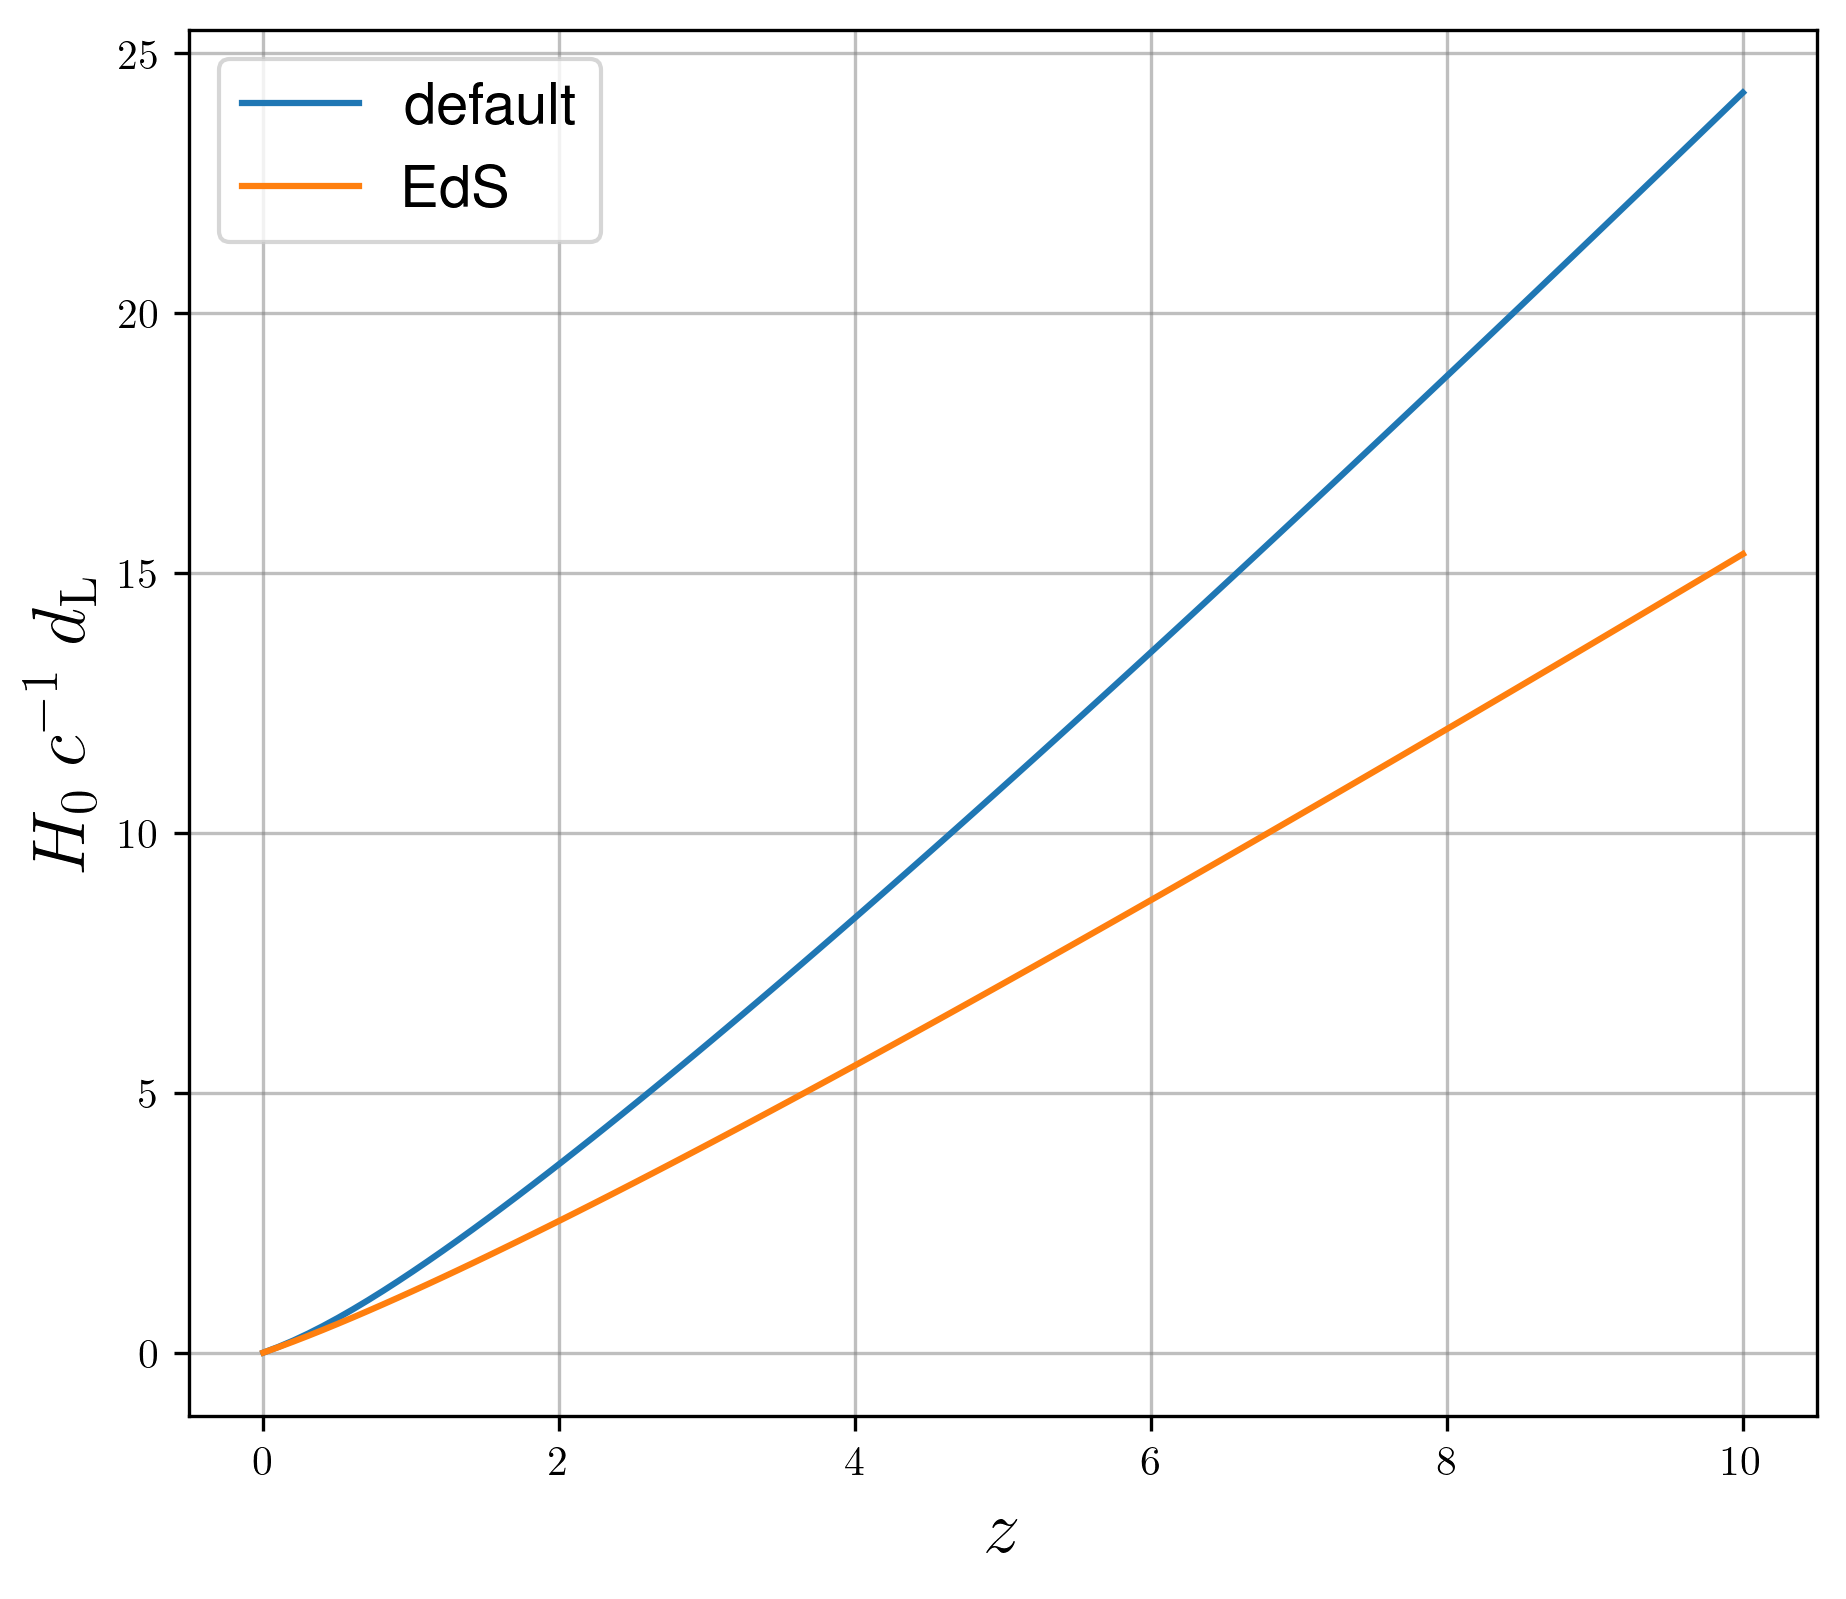
\includegraphics[width=\linewidth]{d_l_plot.png}
							\caption{}
							\label{fig:subfiga}
						\end{subfigure}
						\hfill
						\begin{subfigure}{0.49\textwidth}
							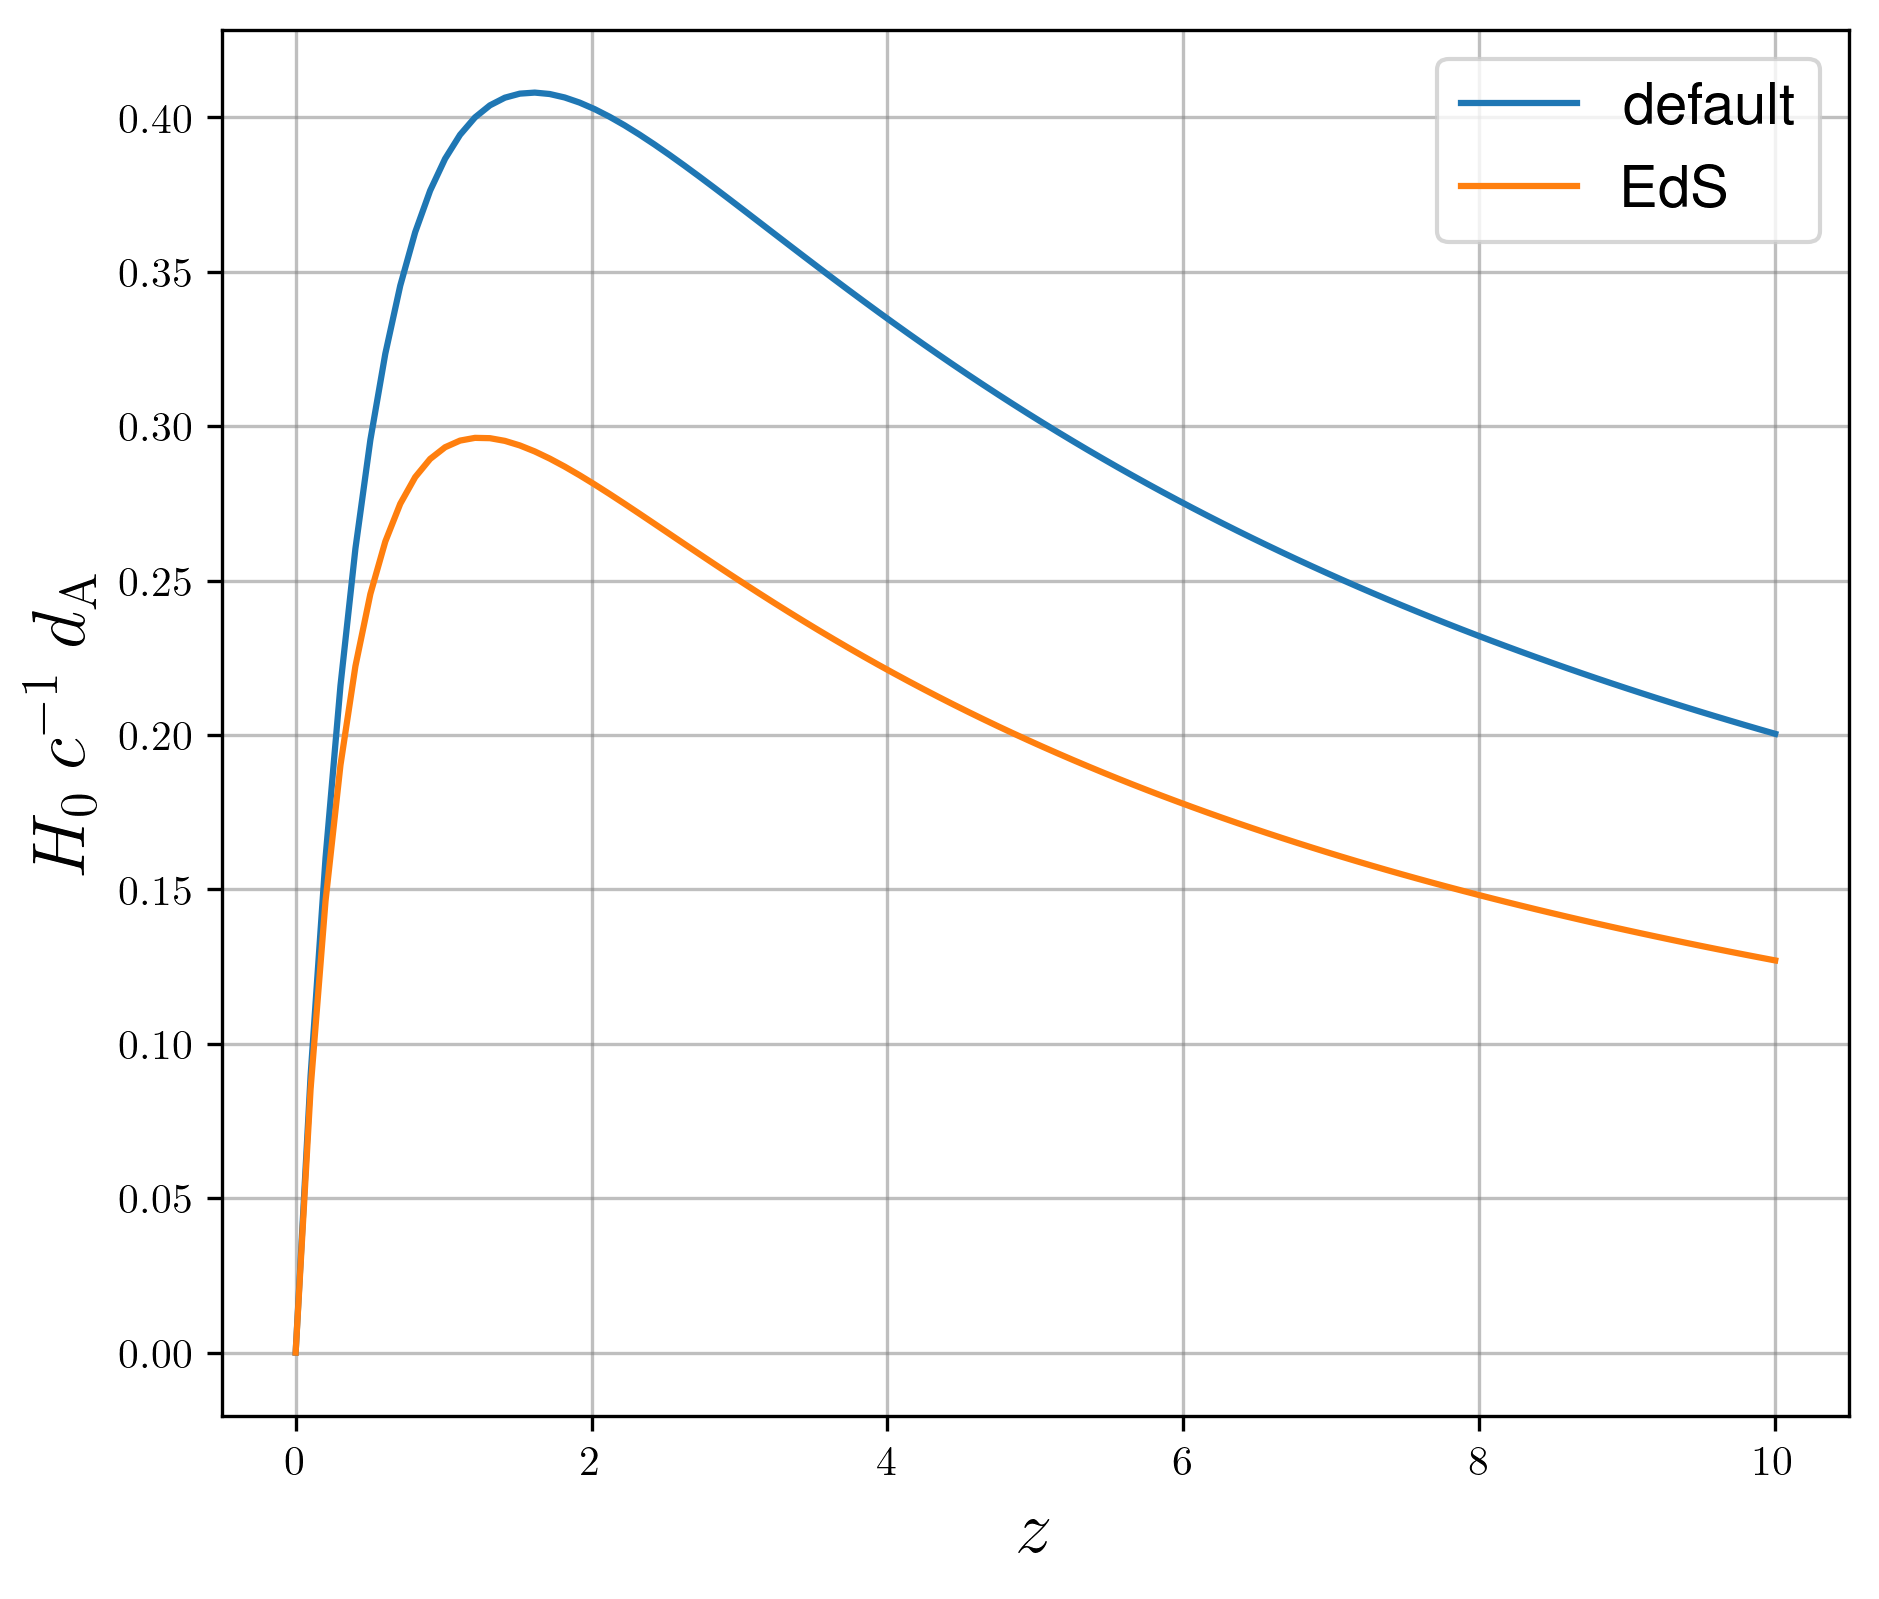
\includegraphics[width=\linewidth]{d_a_plot.png} % Replace with the file name of your second figure
							\caption{}
							\label{fig:subfigb}
						\end{subfigure}
						
						\vspace{0pt}
						
						\caption{The luminosity distance and angular diameter distance as a function of redshift for two different cosmologies.}
						\label{fig:distances}
					\end{minipage}
				} % Close the \fbox
			\end{figure}

			Note in Fig.~\ref{fig:subfigb}, that there is a critical point at $z\approx0.7$.  This corresponds to the epoch when the Universe goes from matter dominated to $\Lambda$ dominated.
			
			\item[Looking Back] In general, we can find the lookback time from the comoving distance (we will explicitly include $c$ to make getting units of time easier): \begin{align*}
				\dif d_\mathrm{M} &= \frac{c}{H(z')} \dif z
			\end{align*} Now, in each differential interval $\dif z$, the distance light must travel is $(1 + z)^{-1} \dif d_\mathrm{M}$.  We get: \begin{align*}
				t_\mathrm{L} &= \frac{1}{H_0} \int_0^z \frac{\dif z'}{(1+z')\left[\Omx{m,0}(1+z')^3 + \Omx{\Lambda}\right]^{1/2}}.
			\end{align*} We use a bisection method to invert this function and solve for $z$ numerically.  See the code in the appendix.  Our results is $\boxed{z = 1.86}$.  This is verified using Astropy.
			
			\item[A $\Lambda$-dominated Universe] We will use the first Friedmann equation to solve for $a(t)$: \begin{align*}
				\left(\frac{\dot{a}}{a}\right)^2 &= \frac{\Lambda}{3}
				\\
				\implies \frac{\dif a}{\dif t} &= \sqrt{\frac{\Lambda}{3}}a
				\\
				\implies a(t) &= Ae^{\sqrt{\Lambda/3}\ t}
			\end{align*} We throw away the negative square root, since we observe $\dot{a}$ to be positive.  To find the age of the Universe, we look for $t$ such that $a(t) = 0$.  But there is no such finite value in this model (i.e., it requires $t=-\infty$).  This implies an infinitely old Universe.

		\end{description} 
	\end{problem}
	
	\begin{problem}{Massive Neutrinos}

	\begin{itemize}
		\item In general, the energy density of a species in an equilibrium gas is given by (e.g., 3.9 in Baumann): \begin{align*}
			\rho &= \frac{g}{(2\pi)^3} \int\dif^3 p\ f(p,T)E(p)
		\end{align*} Where $E(p) = \sqrt{m^2 + p^2}$ and $f(p,T)$ is the distribution function over phase space.  Using the Fermi-Dirac distribution (neutrinos are Fermions), and setting the chemical potential to zero for very early times, we get \begin{align*}
			\rho_\nu = \frac{g_\nu}{2\pi^2}T_\nu^4 \int_0^\infty \dif\xi \frac{\xi^2\sqrt{\xi^2 + m_\nu^2/T_\nu^2}}{\exp\left[ \sqrt{\xi^2 + m_\nu^2/T_\nu^2 } \right] + 1 }
		\end{align*} with $\xi = p/T$.  For relativistic neutrinos, we have $m_\nu\ll T\nu$, and we will use $g=2$ for the spin degrees of freedom for a single neutrino species (e.g. \url{https://physics.stackexchange.com/questions/335061/degrees-of-freedom-of-neutrinos} ). We get \begin{align*}
			\rho_\nu &= \frac{T_\nu^4}{2\pi^2} \int_0^\infty \dif\xi \frac{\xi^2\sqrt{\xi^2 + m_\nu^2/T_\nu^2}}{e^\xi+ 1 }
		\end{align*}
		
		\item In general, we have the expansion $\sqrt{1 + \epsilon^2} = 1 + \frac{\epsilon^2}{2} - \cdots$.  We manipulate as follows: \begin{align*}
			\xi^2\sqrt{\xi^2 + m_\nu^2/T_\nu^2} &= \xi^3\sqrt{1 + \frac{m_\nu^2}{\xi^2T_\nu^2}}
			\\
			&= \xi^3\left[ 1 + \frac{m_\nu^2}{2\xi^2T_\nu^2} + \cdots \right]
			\\
			\implies \rho_\nu &\approx \frac{T_\nu^4}{2\pi^2} \int_0^\infty \dif\xi \frac{\xi^3\left[ 1 + \frac{m_\nu^2}{2\xi^2T_\nu^2} \right]}{e^\xi+ 1 }
			\\
			&= \frac{T_\nu^4}{2\pi^2} \int_0^\infty \dif\xi \frac{\xi^3}{e^\xi+ 1 } + \frac{T_\nu^4}{2\pi^2} \frac{m_\nu^2}{2T_\nu^2} \int_0^\infty \dif\xi \frac{ \xi }{e^\xi+ 1 }
			\\
			&=  \underbrace{\frac{T_\nu^4}{2\pi^2} \frac{7\pi^4}{120}}_{\equiv \rhox{\nu,0}} + \frac{T_\nu^4}{2\pi^2} \frac{m_\nu^2}{2T_\nu^2} \frac{\pi^2}{12}
			\\
			&=  \rhox{\nu,0} \left[ 1 + \frac{5}{7\pi^2 }\frac{m_\nu^2}{T_\nu^2}\right]
		\end{align*}  I used Wolfram Alpha to evaluate the integrals.
		
		\item Let's suppose that in order the be detectable, we require $\rhox{\nu,CMB} \gtrsim 10 \rhox{\nu,0}$.  We will also assume that the relativistic approximation used above is still valid at the epoch of the CMB. We get \begin{align*}
			1 + \frac{5}{7\pi^2 }\frac{m_\nu^2}{T_\nu^2} &\gtrsim 10
			\\
			m_\nu^2 &\gtrsim \frac{63\pi^2}{5}T_\nu^2
			\\
			m_\nu &\gtrsim \sqrt{\frac{63}{5}}\pi T_\nu
			\end{align*} In class, we found that after neutrino decoupling, we have $T_\nu = (4/11)^{1/3}T_\gamma$: \begin{align*}
			m_\nu &\gtrsim \sqrt{\frac{63}{5}}\pi \left(\frac{4}{11}\right)^{1/3} T_{\gamma,0} (1+z)
			\\
			&\approx \sqrt{\frac{63}{5}}\pi \left(\frac{4}{11}\right)^{1/3} 0.235 \text{ meV} \times 1000 
			\\
			&\approx \boxed{1.87 \text{ eV}}
		\end{align*}
		
		\item When a particle goes non-relativistic, its thermal energy becomes much smaller than its rest mass energy.  We look for the redshift at which $m_\nu \sim T_\nu$: \begin{align*}
			T_\nu &\sim m_\nu
			\\
			T_{\nu,0}(1 + z) &\sim m_\nu
			\\
			 \left(\frac{4}{11}\right)^{1/3} T_{\gamma,0} (1+z) &\sim m_\nu
			 \\
			 \implies z_\mathrm{non-rel} &\sim \left(\frac{11}{4}\right)^{1/3} \frac{m_\nu}{0.235 \text{ meV}} - 1
		\end{align*}
	\end{itemize}
		
	\end{problem}
	
	\begin{problem}{Measuring the Expansion History with Standard Candles}
		\begin{itemize}
			\item In order to expand $\chi$ to third order in $z$, we expand the integrand to second order.  Using Mathematica (see code in the appendix), we get: \begin{align*}
				\dif\chi &= \frac{1}{H_0 \left[ \Omx{m,0}(1+z)^3 + \Omx{\Lambda,0} + (1 - \Omx{m,0} - \Omx{\Lambda,0})(1+z)^2 \right]^{1/2}}
				\\
				&\approx \frac{1}{H_0} \left[1 + \frac{-2 + 2 \Omx{\Lambda,0} - \Omx{m,0}}{2} z + \frac{8 - 20 \Omx{\Lambda,0} + 12 \Omx{\Lambda,0}^2 + 4\Omx{m,0}  + 3\Omx{m,0}^2 - 12\Omx{\Lambda,0}\Omx{m,0} }{8} z^2 \right] 
			\end{align*}
			
			\item Now we go back to Python to find the $z$ value at which our third order approximation of $\chi$ diverges from the exact integral by 10\%.  We again implement a bisection method.  See the Python code in the appendix.
			
			We find that this occurs at $\boxed{z=1.204}$.
			
			\item We can use the same procedure to find where the first order approximation $\chi = \frac{z}{H_0}$ (which does not involved the cosmological density parametersdd) differs by the exact integral by at least 10\%.  See the Python code in the appendix.  We find that this occurs at $z=0.386$.
			
			Our statement can be explained using two approaches: \begin{description}
				\item[Intuitively] On an intuitive level, at low redshifts (the local universe), the Hubble parameter is roughly equal to what it is at present day.  We are hardly probing the epochs at which it would be different, so we should only expect to find a constant relationship between recession velocity and distance.  Since the cosmological parameters are related to $H$'s \textit{evolution}, we do not probe them in the local universe.
				
				\item[Mathematically] Using the expansion we just derived, we find that only for $z$ not close to $0$ $\chi$ significantly deviate from the first order expansion, which is sensitive only to $H_0$.  Cosmological density parameters are only probed for higher $z$. 
			\end{description}
		\end{itemize}
	\end{problem}


% Appendix
\appendix
\section{Python code}
%\includepdf[pages=-]{/Users/yaronetokayer/Yale Drive/Classes/PHYS 600/phys600 hw/phys600 hw 3/phys600 hw 3 work nb.pdf}
\section{Mathematica code}
%\includepdf[pages=-]{/Users/yaronetokayer/Yale Drive/Classes/PHYS 600/phys600 hw/phys600 hw 3/phys600 hw 3 work nb.pdf}
\begin{figure}[h!]
	\centering
	\fbox{
		\includegraphics[trim={0 15cm 0 2cm},clip, width=0.95\linewidth]{phys600 hw 3 work nb.pdf}
	}
\end{figure}


\end{document}